% !TEX root = exam.tex
\ifthenelse{\equal{\type}{booklet}}{
\newcommand{\GMMkMeansStudSolA}{
%%%%%%%%%%%%%%%%%%%%%%%%%%%%%%%%%%%%
%%
%%.   YOUR SOLUTION FOR PROBLEM A BELOW THIS COMMENT
%%
%%%%%%%%%%%%%%%%%%%%%%%%%%%%%%%%%%%%
Unsupervised. It doesn't use any kind of label.
}

\newcommand{\GMMkMeansStudSolB}{
%%%%%%%%%%%%%%%%%%%%%%%%%%%%%%%%%%%%
%%
%%.   YOUR SOLUTION FOR PROBLEM A BELOW THIS COMMENT
%%
%%%%%%%%%%%%%%%%%%%%%%%%%%%%%%%%%%%%
By adding a constraint on $r_{ik}$. We would want $r_{ik}$ to be 1 for one, and only one, $k$ for each $i$. So, our constraints can be written as:
\[ r_{ik} \in \{0, 1\} \hspace{0.3cm} \forall i \in \{1, 2, \cdots, D \}, \forall r \in \{1, 2, \cdots, K \} \eqno{(1)}\]
\[ \sum_{k=1}^K r_{ik} = 1 \hspace{0.3cm} \forall i \in \{1, 2, \cdots, D \} \eqno{(2)} \]

Additional to those constraints we could also specify a constraint to ensure the active $k$ is the one corresponding to the closest center:
\[ r_{ik} = \delta\left( k = \argmin_j ||x_i - \mu_j ||^2 \right) \]
}

\newcommand{\GMMkMeansStudSolC}{
%%%%%%%%%%%%%%%%%%%%%%%%%%%%%%%%%%%%
%%
%%.   YOUR SOLUTION FOR PROBLEM A BELOW THIS COMMENT
%%
%%%%%%%%%%%%%%%%%%%%%%%%%%%%%%%%%%%%
Replace the integrity constraint $r_{ik} \in \{0, 1\}$ with $r_{ik} \in [0, 1]$ and ignore the $\delta$ function.
}

\newcommand{\GMMkMeansStudSolD}{
%%%%%%%%%%%%%%%%%%%%%%%%%%%%%%%%%%%%
%%
%%.   YOUR SOLUTION FOR PROBLEM A BELOW THIS COMMENT
%%
%%%%%%%%%%%%%%%%%%%%%%%%%%%%%%%%%%%%
Using the Elbow method\footnote{\url{https://en.wikipedia.org/wiki/Elbow_method_(clustering)}} we can say that $k = 5$ is the best choice because after that the cost decrease is too small.
}

\newcommand{\GMMkMeansStudSolE}{
%%%%%%%%%%%%%%%%%%%%%%%%%%%%%%%%%%%%
%%
%%.   YOUR SOLUTION FOR PROBLEM A BELOW THIS COMMENT
%%
%%%%%%%%%%%%%%%%%%%%%%%%%%%%%%%%%%%%
The basic $k$-means, using Euclidean distance, is certainly not enough to cluster the provided data. The reason for this is that $k$-means tries to find non-overlapping spherical clusters. This is a consequence of using Euclidean distance and not of the $k$-means algorithm per se.  But $k$-means can be used with a whole family of distance functions. There are distance functions that are kernel based that can effectively identify clusters in this data. A Gaussian Kernel based distance is one of them \footnote{\url{https://sites.google.com/site/dataclusteringalgorithms/kernel-k-means-clustering-algorithm}}, this is sometimes referred as Spectral clustering.
}

%\newcommand{\GMMkMeansStudSolF}{
%%%%%%%%%%%%%%%%%%%%%%%%%%%%%%%%%%%%%
%%%
%%%.   YOUR SOLUTION FOR PROBLEM A BELOW THIS COMMENT
%%%
%%%%%%%%%%%%%%%%%%%%%%%%%%%%%%%%%%%%%
%}
 %The students have to fill this file to print the solution
}{
\input{GMMkMeans_OurSolution} %This file will not be provided to students since it contains the solution
}

% Problem Explanation:
% - first argument is the number of points
% - second argument is the title and the text
\examproblem{10}{K-Means\\}


%%%%%%%%%%%%%%%%%%%%%%%%%%%%%%%%%%%%%%
%%%%%  BEGINNING OF SUBPROBLEMS LIST

\begin{enumerate}

 % Subproblem description
\examproblempart{Mention if K-Means is a supervised or an un-supervised method.
 \\}

\bookletskip{0.0}   %in inches

% Solution box
 \framebox[14.7cm][l]{
 \begin{minipage}[b]{14.7cm}
 \inbooklet{Your answer: \GMMkMeansStudSolA}
  
 \solution{\GMMkMeansSolA}
 \end{minipage}
 }
 
  % Subproblem description
\examproblempart{Assume that you are trying to cluster data points $x_{i}$  for $ i \in \{1,2 \dots D\}$ into K clusters each with center $\mu_{k}$  where $ k \in \{1,2, \dots K \}$. The objective function for doing this clustering involves minimizig the euclidean distance between the points and the cluster centers. It is given by  \begin{equation*}
\min\limits_{\mu} \min\limits_{r}\sum\limits_{i \in D} \sum\limits_{k =1}^{K} \frac{1}{2} r_{ik} ||x_{i} -\mu_{k}||_{2}^{2} \\
 \end{equation*} \\ How do you ensure hard assignemnt of one data point to one and only one cluster at a given time? Note: By hard assignment we mean that your are 100 \% sure that a point either belongs or not belongs to a cluster.\\}

\bookletskip{0.0}   %in inches

% Solution box
 \framebox[14.7cm][l]{
 \begin{minipage}[b]{14.7cm}
 \inbooklet{Your answer: \GMMkMeansStudSolB}
  
 \solution{\GMMkMeansSolB }
 \end{minipage}
 }
 
% Subproblem description
\examproblempart{What changes must you do in your answer of part b, to make the hard assingment into a soft assignment? Note: By soft assignment we mean that your are  sure that a point either belongs or not belongs to a cluster with some probability.\\}

\bookletskip{0.0}   %in inches

% Solution box
 \framebox[14.7cm][l]{
 \begin{minipage}[b]{14.7cm}
 \inbooklet{Your answer: \GMMkMeansStudSolC}
  
 \solution{\GMMkMeansSolC}
 \end{minipage}
 }
 
 % Subproblem description
 \examproblempart{Looking at the following plot, what is the best choice for number of clusters?}
  \begin{center}
 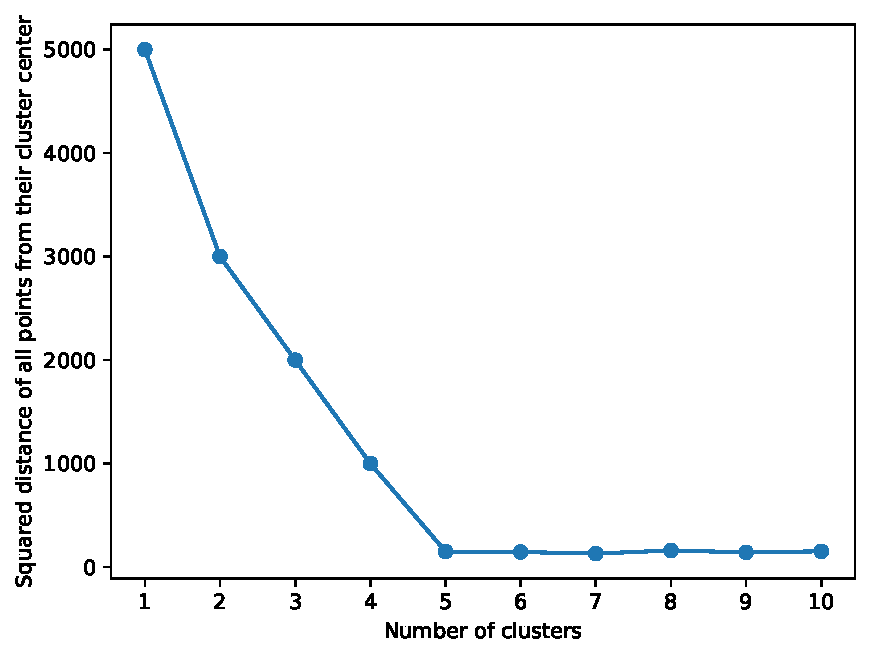
\includegraphics[width=8cm]{fig/cluster.pdf}
 \end{center}
\bookletskip{0.0}   %in inches

% Solution box
 \framebox[14.7cm][l]{
 \begin{minipage}[b]{14.7cm}
 \inbooklet{Your answer: \GMMkMeansStudSolD}
  
 \solution{\GMMkMeansSolD}
 \end{minipage}
 }

% Subproblem description
 \examproblempart{Would K-Means be an effecient algorithm to cluster the following data? Explain your answer in a couple of lines.}
  \begin{center}
 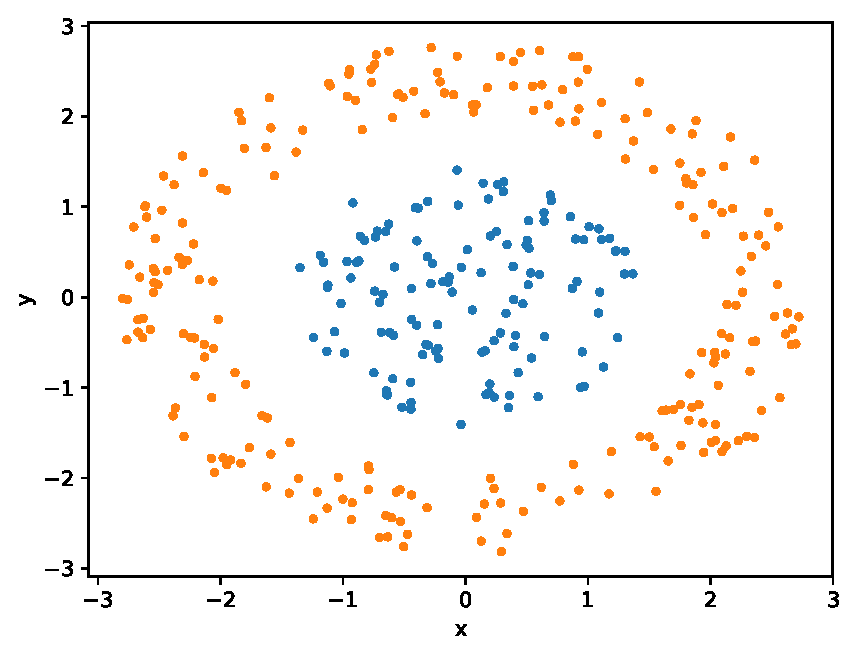
\includegraphics[width=8cm]{fig/concentric.pdf}
 \end{center}
\bookletskip{0.0}   %in inches

% Solution box
 \framebox[14.7cm][l]{
 \begin{minipage}[b]{14.7cm}
 \inbooklet{Your answer: \GMMkMeansStudSolE}
  
 \solution{\GMMkMeansSolE}
 \end{minipage}
 }
 
 %}
 
  %%%%%%%%%%%% END OF SUBPROBLEMS LIST
  
 \end{enumerate}